\documentclass[a4paper, twoside]{article} %document class
%a4paper A4 page format

%extensions
\usepackage[utf8]{inputenc} %input encoding
\usepackage[english]{babel}
\usepackage{ae,lmodern}
\usepackage[T1]{fontenc} %output encoding
\usepackage{amsthm,amsmath,amsfonts,amssymb,mathtools} %math extensions
\usepackage{graphicx} %image extension
\usepackage{xcolor} %color extension
\usepackage{hyperref}
\usepackage[left=1.3cm, right=1.3cm, top=1.3cm, bottom=1.3cm]{geometry} %margins
\usepackage{colortbl}
\graphicspath{ {./img/} }
\usepackage{float} %correct image placement

\usepackage{listings} % Allows adding code

\definecolor{codegreen}{rgb}{0,0.6,0}
\definecolor{codegray}{rgb}{0.5,0.5,0.5}
\definecolor{codepurple}{rgb}{0.58,0,0.82}
\definecolor{backcolour}{rgb}{0.95,0.95,0.92}

\lstdefinestyle{mystyle}{
    backgroundcolor=\color{backcolour},   
    commentstyle=\color{codegreen},
    keywordstyle=\color{magenta},
    numberstyle=\tiny\color{codegray},
    stringstyle=\color{codepurple},
    basicstyle=\ttfamily\footnotesize,
    breakatwhitespace=false,         
    breaklines=true,                 
    captionpos=b,                    
    keepspaces=true,                 
    numbers=left,                    
    numbersep=5pt,                  
    showspaces=false,                
    showstringspaces=false,
    showtabs=false,                  
    tabsize=2
}
\lstset{
        literate=
        {à}{{\`a}}1
        {é}{{\'e}}1
        {è}{{\`e}}1
        {ù}{{\`u}}1,
        style=mystyle
     }

\begin{document}

\begin{figure}[t]
	\begin{minipage}[b]{0.2\linewidth}
		\raggedright 
\includegraphics[scale=0.5]{enib.jpg}
	\end{minipage}\hfill
	\begin{minipage}[b]{0.4\linewidth}	
		\raggedleft 
\includegraphics[scale=0.5]{logo.jpg}
	\end{minipage}
\end{figure}
\begin{titlepage}
\begin{center}
ENIB S4: \\
UE B - Euclidean Space\\
\vspace{2cm}
\huge{\textsl{DTMF Project}\textbf{ : \\
Recognition of a DTMF code within an audio file}}\\
\end{center}
\begin{center}
\rule{\linewidth}{1pt}
\end{center}
\begin{minipage}[t]{0.47\textwidth}
	{\large DE MORAIS Theo}\\
	{\large LE TALLEC NEGRIT Mael}
\end{minipage}\hfill
\begin{minipage}[t]{0.47\textwidth}\raggedleft
	{\large PASCO Florian}\\
	{\large WEBER SEGARRA Yann}
\end{minipage}
\vspace{2.5cm}
\begin{figure}[H]
	\centering 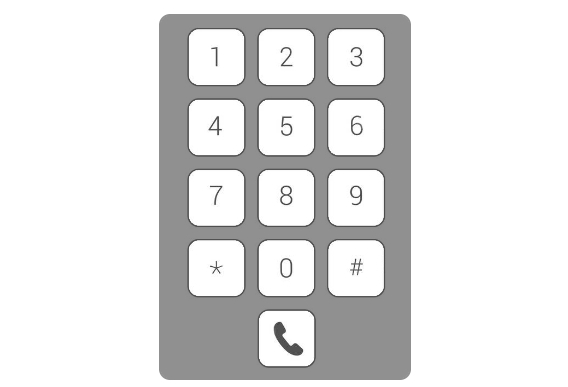
\includegraphics[width=0.8\textwidth]{guardpage.jpg}
\end{figure}
\vspace{0.3cm}
\centering{Version 1.5 : November 2, 2022}
\end{titlepage}

%displaying the table of contents
\tableofcontents
\listoffigures

\newpage

\section{The Problem to Solve}
\subsection{The Problem in its Entirety}
Starting from audio recordings of DTMF codes (explained below), the objective will be to distinguish the number of the pressed key based on the recording.

\subsection{What is DTMF Code?}
A DTMF code is a combination of frequencies used for traditional telephony. The frequencies used are specified in the table below. These codes are emitted when a key on the telephone keypad is pressed, resulting in a distinct sound produced for each key.

\begin{figure}[H]
\begin{center}
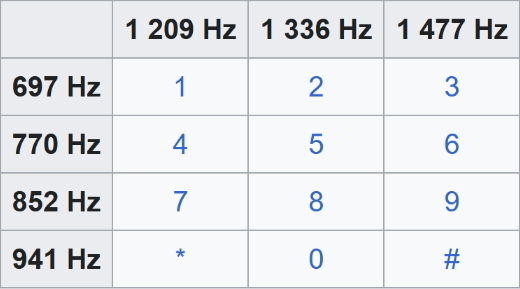
\includegraphics[height=5cm]{img/fig.jpg}\\
\caption{The frequency table associated with each button}
\end{center}
\end{figure}

\subsection{What is an Audio Recording?}
We will be provided with an audio recording that corresponds to the evolution of the amplitude of the sound signal over time.
     % part 1: Problem to solve;
\newpage
\section{Mathematical Modeling and Justification}

\subsection{Vector Space}
To model the mathematical problem, we will work within the set of continuous functions on [0,1]. Here, we will consider a family of vectors composed of sine functions with DTMF code frequencies (697, 770, 852, 941, 1209, 1336, and 1477). 

The functions will take the following form:

$$u1 : [0,1] \rightarrow \mathbb{R}$$
~~~~~~~~~~~~~~~~~~~~~~~~~~~~~~~~~~~~~~~~~~~~~~~~~~~~~~~~~~~~~~~~~~~~~~~~~~~~~~~~~~~~~~~~~~~~~~~~~~~with \( f \) representing the frequencies of our DTMF signals.
$$t \mapsto \sin(f \cdot 2 \cdot \pi \cdot t)$$ 

\subsection{Linear Combination}
Initially, we need to find each coefficient of the linear combination.
\\
To find this linear combination, we can take the inner product of the recording and the 6 functions from our family to determine each coefficient of the linear combination.
\\
\\
The following formula will allow us to compute the inner product:
\[ \int_{0}^{1} u1(t)u2(t) \, \mathrm{d}t\]

We will denote the formula above for the inner product between \( u1 \) and \( u2 \) as \( \langle u1, u2 \rangle \).

\subsection{Demonstration of the Inner Product}

We know that in \( \mathbb{R}^2 \), the inner product of two vectors is defined by:
\newline
\newline 
\[
\begin{pmatrix}
a1 
\\a2
\end{pmatrix}
\cdot
\begin{pmatrix}
b1 
\\b2
\end{pmatrix}
= a1 \cdot b1 + a2 \cdot b2
\]
\newline
\newline
If we generalize for the vectors in our family, we obtain the Riemann sum:
\newline
\newline
\[
= \frac{b-a}{n_{\text{samples}}} \times \sum_{k=1}^{n_{\text{samples}}} f\left(a+\frac{k(b-a)}{n_{\text{samples}}}\right)
\]
With \( f(x) = u1(x) \cdot u2(x) \)
\newline
\newline
If \( f \) is integrable on \([a,b]\), then the Riemann sums converge to the integral of \( f \) over \([a,b]\):
\[
= \int_{a}^{b} f(x) \, dx
\]
In the case where \( a = 0 \) and \( b = 1 \):
\[
= \int_{0}^{1} f(x) \, dx
\]

\subsection{Norm}
We notice that when we take the inner product of two identical vectors, we obtain:
\\
\( \langle u1, u1 \rangle = \frac{1}{2} \)
\\
This means that the norm of our vectors is \( \frac{1}{\sqrt{2}} \) and not 1, so they are not unit vectors. Our family is not normalized, but it is orthogonal.
\\
To address this issue, we need to multiply our functions/vectors by \( \sqrt{2} \) to obtain the correct coefficients corresponding to the components in the DTMF recordings. This amounts to multiplying our inner product by 2.
\\
To revisit the example above, if we want to know the "number of \( u1 \) in \( u1 \)," we need to calculate:
\\
\( \langle \sqrt{2}u1, \sqrt{2}u1 \rangle = 1 \)
\\
\( 2\langle u1, u1 \rangle = 1 \)
\\
There is indeed 1 instance of \( u1 \) in \( u1 \).
Thus, for a signal of the form \( f1 \), we only need to compute the inner product between it and each vector from our family, multiplying our vectors by \( \sqrt{2} \):
\\
\\
\( \langle \sqrt{2}f1, \sqrt{2}u1 \rangle = a \)
\\
\( \langle \sqrt{2}f1, \sqrt{2}u2 \rangle = b \)
\\
\( \langle \sqrt{2}f1, \sqrt{2}u3 \rangle = c \)
\\
\( \langle \sqrt{2}f1, \sqrt{2}u4 \rangle = d \)
\\
\( \langle \sqrt{2}f1, \sqrt{2}u5 \rangle = e \)
\\
\( \langle \sqrt{2}f1, \sqrt{2}u6 \rangle = f \)
\\
\( \langle \sqrt{2}f1, \sqrt{2}u7 \rangle = g \)

Based on the resulting linear combination, we will know which DTMF signals any given signal is composed of, allowing us to deduce the number of the pressed key.

\subsection{The Vectors in Our Family are Orthogonal to Each Other}
Here, we can apply our definition of the inner product to each of our vectors. By doing this, we find that all the inner products are zero. Indeed, our sine functions have arguments of the form \( 2k\pi \), and when we compute our inner product, we ultimately arrive at a sum of \( \sin(2k\pi) \), all of which equal 0.

\subsection{The Family Composed of Sinusoidal Functions (Constructed with DTMF Frequencies) is a Free Family}
\underline{Free Family}: A family of vectors for which the only linear combination that equals the zero vector is the one where all coefficients are zero.

Let us take our DTMF functions \( u1, u2, u3, u4, u5, u6, u7 \) and compute the inner product as follows:
\\
\( \langle u1, a0u0 + a1u1 + a2u2 + a3u3 + a4u4 + a5u5 + a6u6 \rangle = 0 \)
\\
(We assume it is zero according to the property stated above).\\~\\
\( \langle u1, a0u0 \rangle + \langle u1, a1u1 \rangle + \langle u1, a2u2 \rangle + \langle u1, a3u3 \rangle + \langle u1, a4u4 \rangle + \langle u1, a5u5 \rangle + \langle u1, a6u6 \rangle = 0 \)
\\
\( a0 \langle u1, u0 \rangle + a1 \langle u1, u1 \rangle + a2 \langle u1, u2 \rangle + a3 \langle u1, u3 \rangle + a4 \langle u1, u4 \rangle + a5 \langle u1, u5 \rangle + a6 \langle u1, u6 \rangle = 0 \)
\\
If we compute the inner products, we obtain:
\\
\( a0 \times 0 + a1 \times 1 + a2 \times 0 + a3 \times 0 + a4 \times 0 + a5 \times 0 + a6 \times 0 = 0 \)
\\
Thus, we have \( a1 = 0 \) (which is true for \( a1 \) as well as the other coefficients).
\\
Therefore, the only linear combination of these vectors that equals the zero vector is the one where all coefficients are zero, and our family is free.

\subsection{Signal with Phase Shift}

A DTMF signal that we want to decode has a phase shift.
To address this issue, we can express a signal with a phase shift \( \phi \) as follows:
$$\sin(f \cdot 2 \cdot \pi \cdot t + \phi) = \sin(f \cdot 2 \cdot \pi \cdot t) \cos(\phi) + \cos(f \cdot 2 \cdot \pi \cdot t) \sin(\phi)$$
$$= \sin(f \cdot 2 \cdot \pi \cdot t) \cos(\phi) + \sin(f \cdot 2 \cdot \pi \cdot t + \frac{\pi}{2}) \sin(\phi)$$

We can thus consider that a phase-shifted DTMF signal is composed of two identical DTMF signals, one of which is phase-shifted by \( \frac{\pi}{2} \). Both have coefficients \( \cos{\phi} \) and \( \sin{\phi} \).\\

Therefore, for a pulsation \( w_i \):
\\
\( \langle w_i, \sin(w_i t) \rangle = {c_i} \times \cos{\phi} \)\\
\( \langle w_i, \sin(w_i t + \frac{\pi}{2}) \rangle = {c_i} \times \sin{\phi} \)\\

We now want to eliminate the coefficients \( \cos{\phi} \) and \( \sin{\phi} \). To do this, we can add the two inner products and square them:
\\
\( \langle w_i, \sin(w_i t) \rangle^2 + \langle w_i, \sin(w_i t + \frac{\pi}{2}) \rangle^2 = c_i^2 \cos^2(\phi) + c_i^2 \sin^2(\phi) = c_i^2 \)

The coefficient we obtain is squared, but this is not an issue for our application; we only want to find the largest coefficients to recognize the pressed key.
Thus, to decode any phase-shifted DTMF signal, we simply need to enlarge our family of vectors by adding the same vectors but phase-shifted by \( \frac{\pi}{2} \).
     % part 2: Modeling the problem (mathematically);
\newpage
\section{The Strategy for Solving the Problem}
\subsection{Classic Approach}
\subsubsection{Creating the Orthonormal Basis}
The family of vectors (in this case, our sine functions are vectors belonging to the set of continuous functions on [0,1]) that allows us to create DTMF signals is free (as previously demonstrated). We are constrained to discretize each of these functions for analysis since they are of infinite size.

\lstinputlisting[language=Python]{py/createOrthonormalBasis.py}

\subsubsection{Retrieving the DTMF Code to Analyze}
Next, we retrieve the DTMF code transmission that has been recorded for analysis.

\lstinputlisting[language=Python]{py/getCodeFromFile.py}

\subsubsection{Finding the Linear Combination that Created It}
Then, we will find the linear combination that originated the emitted sound. To do this, we will perform an orthogonal projection of our sound onto the orthonormal basis created previously.

\lstinputlisting[language=Python]{py/projectionOrt.py}

To perform this orthogonal projection, we will compute the inner product of our sound with each vector in the basis.

\lstinputlisting[language=Python]{py/scal.py}

\lstinputlisting[language=Python]{py/integrale.py}

\subsubsection{Identifying the Two Main Frequencies}
To form a DTMF code, two sine waves of different frequencies are used. The goal here is to identify these two frequencies.

\lstinputlisting[language=Python]{py/findingMainFrequencies.py}

\subsubsection{Identifying the Associated Digit}
Each combination of vectors is associated with a telephone digit. The question here is to determine which digit it is.

\lstinputlisting[language=Python]{py/whatNumIsIt.py}
     % part 3: Solving the problem;
\section{The Technical Tools Used}
\begin{itemize}
    \item Python (Jupyter Notebook + various libraries)
    \item Vector space
    \item Orthogonality and orthonormal basis
    \item Linear combination
    \item Inner product
    \item Norm
    \item Orthogonal projection
    \item Integral
\end{itemize}
     % part 4: Technical tools used;

\end{document}
